\documentclass[11pt,a4paper]{article}

% -- Encoding & Fonts --
\usepackage[utf8]{inputenc}
\usepackage[T1]{fontenc}
\usepackage{lmodern}

% -- Layout --
\usepackage[margin=1in]{geometry}
\usepackage{setspace}
\onehalfspacing

% -- Mathematics --
\usepackage{amsmath,amssymb}

% -- Graphics & Figures --
\usepackage{graphicx}
\graphicspath{{figures/}}
\usepackage{float}
\usepackage{subcaption}

% -- Tables --
\usepackage{booktabs}
\usepackage{multirow}
\usepackage{tabularx}

% -- Code Listings --
\usepackage{listings}
\lstset{
  basicstyle=\ttfamily\small,
  breaklines=true,
  frame=single,
  numbers=left,
  numberstyle=\tiny\color{gray},
  keywordstyle=\color{blue},
  commentstyle=\color{green!50!black},
  stringstyle=\color{red!60!black},
}

% -- Colors & Hyperlinks --
\usepackage[dvipsnames]{xcolor}
\usepackage[colorlinks=true,linkcolor=blue,citecolor=blue,urlcolor=blue]{hyperref}

% -- Bibliography --
\usepackage[numbers,compress]{natbib}

% -- Misc --
\usepackage{enumitem}

% ==============================================================
% Title
% ==============================================================
\title{%
  \textbf{GrabDrop: Cross-Platform Screenshot Sharing via Hand Gesture Recognition} \\[6pt]
  \large DSAI5201 -- AI and Big Data Computing in Practice \\
  Spring 2026 -- Group Project Report
}
\author{
  WANG Xingxiao \and HE Junpeng \and JI Ying \and CHEN Jinhe
}
\date{\today}

\begin{document}
\maketitle

% -- Abstract --
\begin{abstract}
We present \textbf{GrabDrop}, a cross-platform application that enables
screenshot sharing between devices using natural hand gestures over a local
area network, without relying on cloud services, user accounts, or device
pairing. Users perform a \emph{grab} gesture (closing the hand from palm to
fist) to capture and broadcast a screenshot, and a \emph{release} gesture
(opening the hand from fist to palm) on another device to receive it. The
system additionally supports \emph{swipe} gestures for remote page scrolling.
At its core, GrabDrop employs a lightweight Temporal Convolutional Network
(TCN) trained on 144-dimensional hand landmark features extracted via
MediaPipe. The model is optimized for edge deployment through structured
pruning (1.9$\times$ compression) and INT8 quantization, resulting in a final
model size of approximately 140\,KB. We develop native clients for both
Android (Kotlin/Jetpack Compose) and Desktop (Python) with a unified UDP/TCP
network protocol enabling seamless cross-platform interoperability.
Experimental results demonstrate an overall test accuracy of 89.66\%
across five gesture classes, with the optimized model running in
real-time on commodity hardware. The source code is publicly available\cite{grabdrop}.
\end{abstract}

% -- Sections (one file per section for team collaboration) --
\section{Introduction}
\label{sec:introduction}

The proliferation of multi-device computing environments has created a
persistent need for seamless content sharing across heterogeneous platforms.
While cloud-based solutions such as AirDrop~\cite{apple2023airdrop},
Google Nearby Share~\cite{google2023nearby}, and Huawei Share
address this need, they typically require vendor lock-in, account
authentication, or explicit pairing protocols. In scenarios
where privacy, latency, and simplicity are paramount---for example, in
enterprise environments behind firewalls, classroom demonstrations, or
offline field deployments---a lightweight, infrastructure-free alternative
is desirable.

Concurrently, advances in hand gesture recognition have made contactless
human--computer interaction increasingly practical. MediaPipe
Hands~\cite{zhang2020mediapipe} provides robust real-time hand landmark
detection on commodity hardware, while lightweight neural architectures
such as Temporal Convolutional Networks (TCNs)~\cite{bai2018empirical,
lea2017temporal} enable accurate temporal pattern recognition with
minimal computational overhead.

In this work, we present \textbf{GrabDrop}, a system that bridges these
two domains by enabling \emph{gesture-driven screenshot sharing} over a
local area network. The key idea is intuitive: a user \emph{grabs} a
screenshot by closing their hand (palm to fist), and another user
\emph{releases} it by opening their hand (fist to palm) on a different
device. The transfer happens instantly over WiFi with no cloud, no
accounts, and no pairing required. Additionally, swipe gestures (hand
moving up or down) enable remote page scrolling.

\subsection{Contributions}

The main contributions of this project are as follows:

\begin{enumerate}[leftmargin=*]
  \item \textbf{End-to-end gesture recognition pipeline.} We design a
    complete pipeline from raw video capture through hand landmark
    extraction (MediaPipe), feature engineering (144~dimensions),
    temporal classification (TCN), and gesture event emission, operating
    in real-time with a two-stage (Idle/Wakeup) power-aware detection
    scheme.

  \item \textbf{Model optimization for edge deployment.} We apply
    structured pruning (30\% channel reduction, yielding
    1.9$\times$~compression from 87K to 46K parameters) followed by
    INT8 static quantization, producing a deployment-ready ONNX model
    of approximately 140\,KB with minimal accuracy degradation.

  \item \textbf{Cross-platform application.} We implement native clients
    for Android (Kotlin/Jetpack~Compose) and Desktop (Python), sharing a
    unified UDP/TCP network protocol for device discovery and screenshot
    transfer. Both platforms support dual detection backends (Neural
    Network and Legacy rule-based) with automatic fallback.

  \item \textbf{Comprehensive data augmentation.} We employ seven
    augmentation techniques including temporal reversal with label
    remapping, expanding a small video dataset into thousands of
    training samples.
\end{enumerate}

The remainder of this report is organized as follows:
Section~\ref{sec:related_work} reviews related work;
Section~\ref{sec:data} describes data collection and preprocessing;
Section~\ref{sec:methodology} details the gesture detection methodology
and TCN architecture;
Section~\ref{sec:training} presents the training procedure;
Section~\ref{sec:deployment} covers model optimization and deployment;
Section~\ref{sec:application} describes the cross-platform application
design;
Section~\ref{sec:results} reports experimental results; and
Section~\ref{sec:conclusion} concludes with future directions.

\section{Related Work}
\label{sec:related_work}

\subsection{Hand Gesture Recognition}

Hand gesture recognition has been extensively studied using both
vision-based and sensor-based approaches. Early methods relied on colored
gloves or depth sensors~\cite{rautaray2015vision}, while modern
approaches leverage deep learning on RGB camera input.
MediaPipe~\cite{zhang2020mediapipe} provides a lightweight hand
landmark detection model that extracts 21 3D keypoints in real-time,
forming the basis for many downstream gesture classification systems.

For temporal gesture classification, Recurrent Neural Networks (RNNs)
and Long Short-Term Memory (LSTM) networks have been widely
used~\cite{pigou2018gesture}. However, Temporal Convolutional Networks
(TCNs)~\cite{bai2018empirical, lea2017temporal} have emerged as a
competitive alternative, offering parallelizable training, stable
gradient flow via residual connections, and flexible receptive fields
through dilated causal convolutions. Lea et al.~\cite{lea2017temporal}
demonstrated that TCNs outperform LSTMs on action segmentation tasks
while being significantly faster to train.

\subsection{Model Compression for Edge Deployment}

Deploying deep learning models on resource-constrained devices (e.g.,
smartphones, embedded systems) requires model compression techniques.
Structured pruning~\cite{li2017pruning} removes entire convolutional
filters, producing genuinely smaller models without requiring sparse
hardware support. Network quantization~\cite{jacob2018quantization}
reduces numerical precision from 32-bit floating point to 8-bit
integers, achieving approximately $4\times$ memory reduction. The ONNX
Runtime~\cite{onnxruntime} provides a portable inference engine that
supports both pruned and quantized models across diverse hardware
platforms.

\subsection{Contactless Device Interaction}

Gesture-based device interaction has been explored in various contexts.
Gesture control for smart TVs~\cite{samsung2013gesture}, automotive
interfaces~\cite{ohn2014hand}, and augmented reality
headsets~\cite{meta2023hand} demonstrates the practical applicability
of hand gesture recognition. However, using gestures specifically for
\emph{cross-device content transfer} remains relatively unexplored.
Existing wireless sharing solutions such as Apple AirDrop, Google Nearby
Share, and Huawei Share rely on explicit user actions (button taps,
device selection) rather than natural gestures. GrabDrop fills this gap
by combining real-time gesture recognition with a zero-configuration
network protocol.

\section{Data Collection and Preprocessing}
\label{sec:data}

\subsection{Dataset}

We collected a custom dataset of hand gesture video clips recorded via
webcam and phone cameras. Each clip captures a single gesture instance
and is labeled as one of five classes: \texttt{grab} (palm $\to$ fist),
\texttt{release} (fist $\to$ palm), \texttt{swipe\_up},
\texttt{swipe\_down}, and \texttt{noise} (invalid/unrecognized motions).
The dataset is split into training and test sets, organized by class.

\subsection{Hand Landmark Extraction}

For each frame of a video clip, we use MediaPipe Hand
Landmarker~\cite{zhang2020mediapipe} to extract 21~3D hand landmarks,
producing a 63-dimensional raw feature vector per frame
($21 \times 3$ coordinates: $x$, $y$, $z$). Coordinates $x$ and $y$
are normalized to $[0, 1]$ relative to the image dimensions, and $z$
represents depth relative to the wrist. If MediaPipe fails to detect a
hand in a given frame, the result is marked as missing. Videos with
fewer than 10\% valid frames are discarded as low-quality.

\subsection{Missing Frame Interpolation}

Because MediaPipe may fail to detect hands in certain frames (due to
motion blur, occlusion, or poor lighting), we apply linear interpolation
to fill gaps between valid detections. For missing frames at the
boundaries of a video, linear extrapolation from the two nearest valid
frames is used. This ensures a complete landmark sequence without
discontinuities.

\subsection{Temporal Resampling}

Since gesture videos vary in duration, we resample every landmark
sequence to a fixed length of $T = 30$~frames using linear
interpolation along the time axis. This standardization ensures
uniform input dimensions for the neural network regardless of the
original video frame rate or gesture speed.

\subsection{Feature Engineering}
\label{subsec:features}

Raw landmark coordinates are not ideal inputs for classification, as they
are sensitive to hand position in the frame and distance from the camera.
We compute a 144-dimensional feature vector per frame from the 63~raw
values, as summarized in Table~\ref{tab:features}.

\begin{table}[ht]
\centering
\caption{Feature engineering: 63 raw landmark values $\to$ 144
  engineered features per frame.}
\label{tab:features}
\begin{tabular}{@{}llp{6.5cm}@{}}
\toprule
\textbf{Feature Group} & \textbf{Dims} & \textbf{Description} \\
\midrule
Normalized landmarks & 63 & Landmarks relative to the wrist, divided by palm size (distance from wrist to middle finger MCP). Translation- and scale-invariant. \\
Velocity & 63 & Frame-to-frame difference of normalized landmarks. Captures motion direction and speed. \\
Wrist velocity & 3 & Absolute wrist position change between frames. Critical for swipe detection. \\
Finger pair distances & 10 & Euclidean distances between all $\binom{5}{2}=10$ fingertip pairs. Measures hand openness. \\
Finger curl angles & 5 & Bending angle (via $\arccos$) for each of the 5~fingers. Distinguishes extended from curled. \\
\midrule
\textbf{Total} & \textbf{144} & \\
\bottomrule
\end{tabular}
\end{table}

\subsection{Data Augmentation}

To expand our limited video dataset, we apply seven augmentation
techniques during preprocessing:

\begin{enumerate}[leftmargin=*]
  \item \textbf{Time crops:} Extract sub-sequences at different
    start/end positions (up to 9 crops per video).
  \item \textbf{Jitter:} Add small Gaussian noise
    ($\sigma = 0.003$) to landmark coordinates (3~variants).
  \item \textbf{Rotation:} Rotate landmarks around the wrist by
    $\{-15, -10, -5, +5, +10, +15\}$~degrees (6~variants).
  \item \textbf{Scale:} Scale hand size by factors
    $\{0.85, 0.9, 1.1, 1.15\}$ relative to the wrist (4~variants).
  \item \textbf{Time warp:} Non-linearly stretch/compress along the
    time axis (2~variants).
  \item \textbf{Speed change:} Uniformly speed up or slow down the
    gesture by a random factor in $[0.8, 1.2]$ (2~variants).
  \item \textbf{Time reversal with label remapping:} Reversing a
    \texttt{grab} produces a valid \texttt{release} and vice versa;
    reversing \texttt{swipe\_up} yields \texttt{swipe\_down}
    (1~variant with corrected label).
\end{enumerate}

This pipeline yields approximately 20--30 augmented samples per
original video. Additionally, online augmentation (50\% jitter,
30\% time warp) is applied stochastically during training for
further regularization.

\subsection{Normalization Statistics}

We compute per-feature mean $\mu_d$ and standard deviation $\sigma_d$
across all training samples and all time steps. During both training
and inference, features are $z$-score normalized:
\begin{equation}
  \hat{x}_d = \frac{x_d - \mu_d}{\sigma_d + \epsilon}, \quad
  \epsilon = 10^{-8}.
  \label{eq:normalize}
\end{equation}
The statistics are serialized alongside the model for deployment
(see Section~\ref{sec:deployment}).

\section{Methodology}
\label{sec:methodology}

\subsection{System Overview}

GrabDrop employs a two-stage gesture detection pipeline shared across
both the Neural Network (TCN) and Legacy (rule-based) backends
(Figure~\ref{fig:two-stage}):

\begin{enumerate}[leftmargin=*]
  \item \textbf{IDLE stage} ($\sim$10\,FPS): Low-power scanning for
    hand presence. A sliding window of 10~frames tracks hand detection
    counts; when $\geq 8$ frames contain a detected hand, the system
    transitions to the WAKEUP stage.
  \item \textbf{WAKEUP stage} ($\sim$30\,FPS): High-precision gesture
    classification. Runs for at most 2~seconds before timing out and
    returning to IDLE.
\end{enumerate}

\begin{figure}[ht]
  \centering
  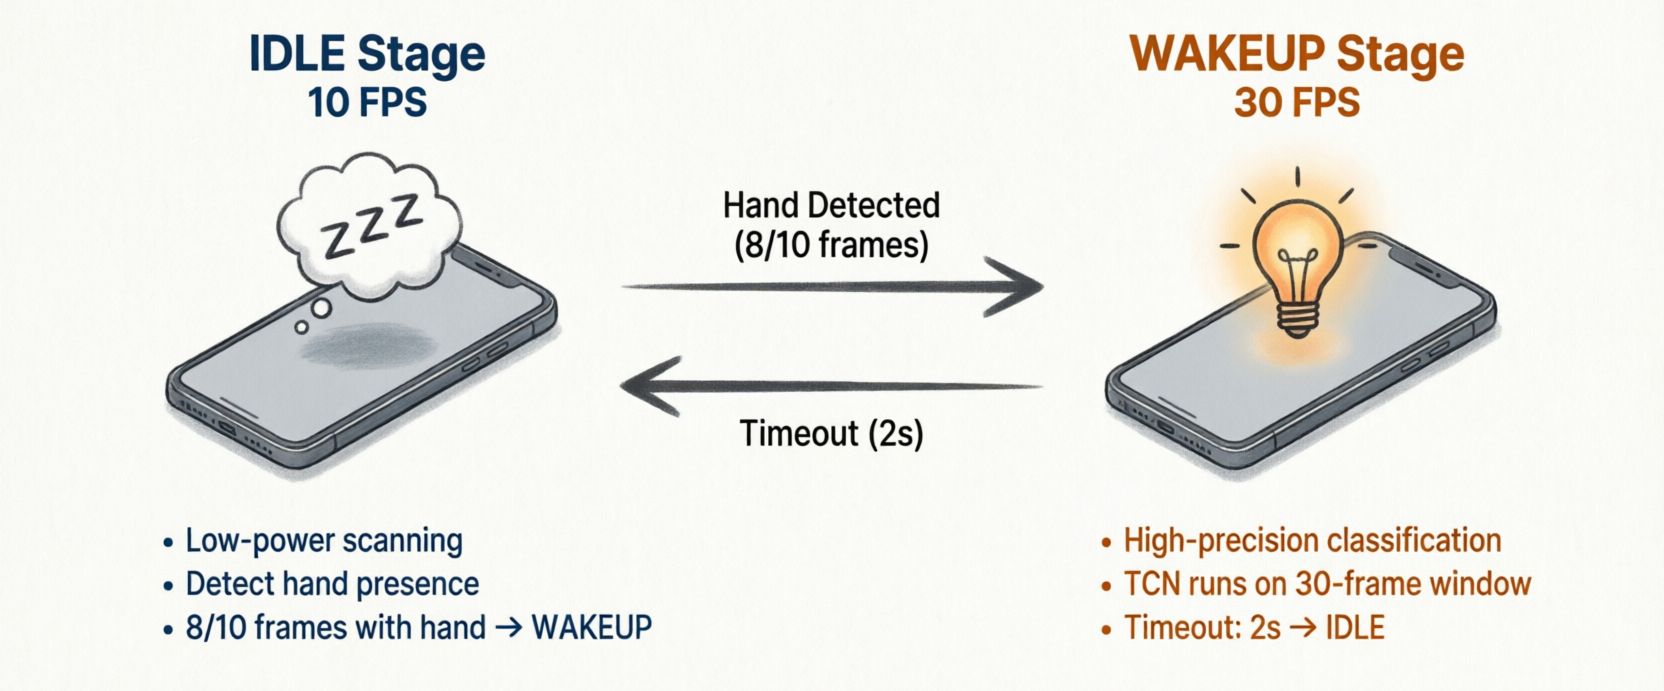
\includegraphics[width=0.85\linewidth]{two-stage-pipeline}
  \caption{Two-stage detection pipeline: IDLE (low power) $\to$ WAKEUP
    (high precision). The system spends most time in IDLE, consuming
    minimal CPU.}
  \label{fig:two-stage}
\end{figure}

\subsection{Neural Network Backend: Temporal Convolutional Network}

The core gesture classifier is a Temporal Convolutional Network
(TCN)~\cite{bai2018empirical, lea2017temporal} that classifies a
30-frame sliding window of 144-dimensional feature vectors into one
of five classes.

\subsubsection{Causal Dilated Convolutions}

The TCN uses \emph{causal} 1D convolutions: the output at time $t$
depends only on inputs at times $\leq t$, which is essential for
real-time inference where future frames are unavailable. \emph{Dilated}
convolutions skip intermediate time steps to expand the receptive field
without increasing parameters:

\begin{equation}
  y(t) = \sum_{i=0}^{k-1} w(i) \cdot x(t - d \cdot i),
  \label{eq:dilated_conv}
\end{equation}
where $k$ is the kernel size, $d$ is the dilation factor, and $w$
denotes learned filter weights. With dilations $\{1, 2, 4\}$, the
network captures local, medium-range, and long-range temporal patterns
respectively.

\subsubsection{Residual Blocks}

Each processing stage uses residual blocks with the structure:
\[
  \text{output} = \text{ReLU}\!\bigl(\mathcal{F}(x) + x\bigr),
\]
where $\mathcal{F}$ denotes two stacked causal convolutions with batch
normalization and dropout ($p=0.15$). The skip connection $+\,x$
facilitates gradient flow and enables the block to learn incremental
refinements. When the channel dimension changes, a $1\!\times\!1$
convolution serves as the skip projection.

\subsubsection{Model Architecture}

The full GestureTCN architecture comprises:

\begin{enumerate}[leftmargin=*]
  \item \textbf{Stem}: $1\!\times\!1$ convolution projecting 144 input
    features to 48 channels, followed by batch normalization and ReLU.
  \item \textbf{Block~1}: Residual block, $k\!=\!3$, dilation $d\!=\!1$
    (48 channels, local patterns).
  \item \textbf{Block~2}: Residual block, $k\!=\!3$, $d\!=\!2$
    (48 channels, medium-range patterns).
  \item \textbf{Block~3}: Channel block, $k\!=\!3$, $d\!=\!4$
    (48$\to$64 channels, long-range patterns).
  \item \textbf{Block~4}: Residual block, $k\!=\!3$, $d\!=\!1$
    (64 channels, refinement).
  \item \textbf{Pooling}: Adaptive average pooling across the time
    dimension, producing a single 64-dim vector.
  \item \textbf{Classification head}: Two fully connected layers
    ($64 \to 32 \to 5$) with ReLU and dropout.
\end{enumerate}

The model contains only \textbf{87,077 parameters} (0.34\,MB),
making it suitable for mobile and embedded deployment. Weights are
initialized using Kaiming normal initialization~\cite{he2015delving}.

\subsection{Legacy Backend: Rule-Based Detection}

As a fallback, GrabDrop includes a rule-based detection mode that
requires no trained model. For each frame, it computes a finger curl
ratio:
\begin{equation}
  r_i = \frac{\|\text{tip}_i - \text{wrist}\|}
             {\|\text{mcp}_i - \text{wrist}\|},
  \label{eq:curl_ratio}
\end{equation}
where $\text{tip}_i$ and $\text{mcp}_i$ are the fingertip and
metacarpophalangeal joint of finger $i$ (excluding the thumb). A finger
is classified as \emph{extended} if $r_i > 1.3$ and \emph{curled} if
$r_i < 0.9$. A hand is classified as \textsc{palm} when $\geq 3$
fingers are extended, and \textsc{fist} when $\geq 3$ are curled.

In the WAKEUP stage, 8~consecutive frames of the target state
(e.g., \textsc{fist} following a \textsc{palm} trigger) confirm a
\texttt{grab} gesture. Swipe detection uses frame-to-frame wrist
$y$-velocity and cumulative displacement against configurable
thresholds.

If the Neural Network backend is selected but fails to load (e.g.,
missing ONNX file), the system automatically falls back to Legacy
mode.

\section{Model Training}
\label{sec:training}

\subsection{Training Setup}

The GestureTCN model is trained using PyTorch on a single GPU.
Table~\ref{tab:hyperparams} summarizes the key hyperparameters.

\begin{table}[ht]
\centering
\caption{Training hyperparameters.}
\label{tab:hyperparams}
\begin{tabular}{@{}ll@{}}
\toprule
\textbf{Hyperparameter} & \textbf{Value} \\
\midrule
Batch size & 32 \\
Maximum epochs & 300 \\
Optimizer & AdamW \\
Learning rate & $2 \times 10^{-3}$ \\
Weight decay & $1 \times 10^{-3}$ \\
LR scheduler & Cosine annealing ($\eta_{\min} = 10^{-5}$) \\
Gradient clipping & Max norm 2.0 \\
Early stopping patience & 40 epochs \\
\bottomrule
\end{tabular}
\end{table}

\subsection{Loss Function}

We use cross-entropy loss with label smoothing ($\alpha = 0.1$) and
inverse-frequency class weights:
\begin{equation}
  \mathcal{L} = -\sum_{c=1}^{C} w_c \, \tilde{y}_c \log p_c,
  \label{eq:loss}
\end{equation}
where $\tilde{y}_c = (1-\alpha) \cdot y_c + \alpha / C$ is the
smoothed label, $p_c$ is the predicted probability via softmax, and
$w_c$ is the class weight computed as $w_c = N / (C \cdot n_c)$ with
$n_c$ being the number of samples in class $c$. Label smoothing
prevents overconfident predictions and improves generalization, while
class weights address the moderate class imbalance in the dataset
(e.g., \texttt{swipe\_up} has the fewest training samples and
receives weight 1.259 versus 0.867 for \texttt{release}).

\subsection{Class Balancing}

In addition to weighted loss, we employ a \texttt{WeightedRandomSampler}
that assigns sampling probability inversely proportional to class
frequency. This ensures each class is sampled approximately equally
within each epoch, further mitigating class imbalance.

\subsection{Online Augmentation}

Beyond the offline augmentation described in
Section~\ref{sec:data}, the PyTorch \texttt{Dataset} applies
stochastic augmentation at each access:
\begin{itemize}[leftmargin=*]
  \item Coordinate jitter ($\sigma = 0.002$) with 50\% probability.
  \item Time warping with 30\% probability.
\end{itemize}
This means the model sees slightly different variants of each sample
every epoch, further improving generalization.

\subsection{Training Dynamics}

Training terminated after 68~epochs via early stopping, with the best
test accuracy of 89.66\% achieved at epoch~28.
Figure~\ref{fig:training_curves} shows the training and test loss/accuracy curves. The cosine annealing schedule
smoothly reduces the learning rate from $2\!\times\!10^{-3}$ to
$10^{-5}$, enabling fine-grained convergence in later epochs.

\begin{figure}[ht]
  \centering
  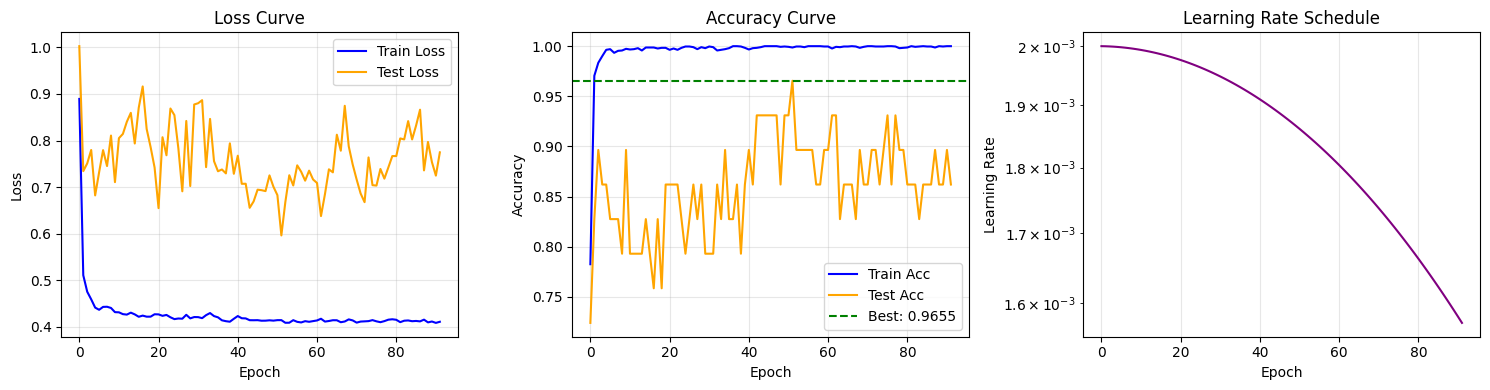
\includegraphics[width=0.95\linewidth]{training_curves}
  \caption{Training curves: loss (left) and accuracy (right) over
    68~epochs. Early stopping was triggered at epoch~68 with the best
    model saved at epoch~28.}
  \label{fig:training_curves}
\end{figure}

\section{Model Optimization and Deployment}
\label{sec:deployment}

Deploying the trained GestureTCN on edge devices requires reducing both
model size and inference latency. We apply a three-step optimization
pipeline: structured pruning, ONNX export, and INT8 quantization.

\subsection{Structured Pruning}

Unlike unstructured pruning (which zeroes individual weights but
maintains tensor dimensions), \emph{structured pruning} removes entire
convolutional channels, producing a genuinely smaller
model~\cite{li2017pruning}. We apply a uniform channel reduction ratio
of 30\%, with channel counts rounded to multiples of~8 for SIMD
alignment:

\begin{table}[ht]
\centering
\caption{Channel dimensions before and after structured pruning.}
\label{tab:pruning}
\begin{tabular}{@{}lcc@{}}
\toprule
\textbf{Component} & \textbf{Original} & \textbf{Pruned} \\
\midrule
Stem channels & 48 & 32 \\
Mid-block channels & 48 & 32 \\
Output channels & 64 & 48 \\
Head hidden units & 32 & 24 \\
\midrule
Total parameters & 87,077 & 45,877 \\
Model size (FP32) & 0.34\,MB & 0.18\,MB \\
Compression ratio & 1.0$\times$ & 1.9$\times$ \\
\bottomrule
\end{tabular}
\end{table}

The pruned model is a new instance of \texttt{GestureTCN} with reduced
channel dimensions. It is fine-tuned for 100~epochs using the
same dataset and a lower learning rate ($10^{-3}$), achieving a test
accuracy of 89.66\%.

\subsection{ONNX Export}

We export the pruned model to ONNX (Open Neural Network
Exchange)~\cite{onnxruntime} format using PyTorch's tracing-based
exporter. The export specification includes a dynamic batch axis to accommodate variable batch sizes at inference time, opset version 18 to ensure compatibility with modern ONNX Runtime versions, and named input and output tensors where the input tensor is designated as \texttt{``input''} with shape $[B, 144, 30]$ and the output tensor is designated as \texttt{``logits''} with shape $[B, 5]$.
Model validity is verified using \texttt{onnx.checker.check\_model()}.

\subsection{INT8 Static Quantization}

We apply static quantization via ONNX
Runtime~\cite{jacob2018quantization}, converting FP32 weights to
signed 8-bit integers through a three-phase process. In the calibration phase, real training data is fed through the FP32 ONNX model to observe the range of activation values at each layer. Subsequently, in the scale computation phase, per-tensor scale and zero-point values are computed to map FP32 ranges to INT8 according to the formula $x_{\text{int8}} = \text{round}(x_{\text{fp32}} / s) + z$. Finally, in the QDQ insertion phase, Quantize-Dequantize (QDQ) nodes are inserted into the computation graph, enabling the runtime to fuse quantized operations for optimal performance.

\paragraph{Quantization Benefits.}
The primary benefit of INT8 quantization for this model is \emph{inference acceleration} rather than size reduction. On mobile CPUs and NPUs, INT8 operations are typically 2--4$\times$ faster than FP32 operations due to specialized hardware support and reduced memory bandwidth. While quantization theoretically reduces weight storage by 4$\times$ (32-bit to 8-bit), the QDQ format adds metadata overhead for each quantized operation. For small models ($<$100\,KB), this overhead can offset weight compression gains---our quantized model is 0.14\,MB compared to the FP32 ONNX model's 0.09\,MB. This phenomenon is well-documented for compact neural networks where the fixed overhead of quantization metadata dominates the variable savings from weight compression.

\subsection{Deployment Configuration}

A \texttt{config.json} file is generated alongside the ONNX model,
containing all information required for inference on edge devices:
class names, sequence length, feature dimension, normalization
statistics ($\boldsymbol\mu$ and $\boldsymbol\sigma$ vectors of
dimension~144), landmark topology (finger chains, joint pairs,
tip/base indices), and pruned channel dimensions. This ensures
complete self-containment of the deployed artifact.

\subsection{Optimization Summary}

Table~\ref{tab:optimization_summary} summarizes the full optimization
pipeline.

\begin{table}[ht]
\centering
\caption{Model optimization pipeline summary.}
\label{tab:optimization_summary}
\begin{tabular}{@{}lcccc@{}}
\toprule
\textbf{Stage} & \textbf{Params} & \textbf{Size} & \textbf{Accuracy} & \textbf{Format} \\
\midrule
Original (FP32) & 87,077 & 0.34\,MB & 89.66\% & PyTorch \\
Pruned (FP32) & 45,877 & 0.18\,MB & 89.66\% & PyTorch \\
Original ONNX (FP32) & 87,077 & 0.09\,MB & 89.66\% & ONNX \\
Pruned ONNX (FP32) & 45,877 & 0.09\,MB & 89.66\% & ONNX \\
Pruned + Quantized (INT8) & 45,877 & 0.14\,MB & 89.66\% & ONNX \\
\bottomrule
\end{tabular}
\end{table}

The ONNX format produces more compact files than PyTorch's serialization format. Notably, the INT8 quantized model is slightly larger than the FP32 ONNX models due to QDQ node overhead, as discussed above. For deployment, we select the quantized model primarily for its faster inference speed on mobile hardware rather than size reduction.

\section{Cross-Platform Application Design}
\label{sec:application}

GrabDrop is implemented as two native clients---Android and
Desktop---that interoperate seamlessly via a shared network protocol.

\subsection{Android Client}

The Android client is built with Kotlin and Jetpack Compose
(Material~3), targeting Android~10+ (API~29). The architecture incorporates several key components: a foreground service designated \texttt{GrabDropService} that hosts the camera pipeline, gesture detector, network manager, and overlay manager while operating independently of the UI lifecycle; CameraX integration providing the \texttt{ImageAnalysis} use case for front camera frames at configurable frame rates; MediaPipe tasks-vision (v0.10.14) for hand landmark detection on each camera frame, operating in \texttt{VIDEO} mode to enable temporal tracking; ONNX Runtime Android (v1.20.0) for executing the pruned and quantized TCN model during gesture classification; MediaProjection for capturing screenshots upon \texttt{GRAB} events; and window-manager-based overlay animations that provide visual feedback including a flash effect on grab, a ripple effect on release, and a wakeup indicator.

\subsection{Desktop Client}

The Desktop client is a Python CLI application compatible with Linux,
macOS, and Windows. Its architecture mirrors the Android client,
incorporating OpenCV for camera capture via \texttt{VideoCapture}, MediaPipe Python (v0.10.14) for hand landmark detection, ONNX Runtime ($\geq$1.17.0) for TCN inference, platform-specific screenshot tools including \texttt{spectacle} for KDE/Wayland, \texttt{grim} for generic Wayland, \texttt{scrot} for X11, \texttt{screencapture} for macOS, or \texttt{mss} for Windows, and Tkinter-based overlays for visual feedback indicators.

\subsection{Network Protocol}

Both clients share a unified zero-configuration network protocol
operating over the local area network:

\subsubsection{Device Discovery (UDP)}

Each device broadcasts a JSON heartbeat message every 3~seconds via
both multicast (\texttt{239.255.77.88:9877}) and broadcast
(\texttt{255.255.255.255:9877}) for reliability. Messages contain a
unique device ID, device name, and timestamp. Devices not heard from
for 10~seconds are removed from the discovery table.

\subsubsection{Screenshot Transfer (UDP + TCP)}

Upon a \texttt{GRAB} event, the system initiates a three-phase transfer protocol. First, the sender captures a screenshot and starts a TCP server on a random port. Second, a \texttt{SCREENSHOT\_READY} JSON message is broadcast via UDP, containing the TCP port and file size. Third, when a receiver performs a \texttt{RELEASE} gesture, it connects to the sender's TCP server, sends the command \texttt{"GET\textbackslash n"}, and receives a 4-byte big-endian length header followed by the raw PNG data.

\subsubsection{Retroactive Matching}

To handle network latency, the protocol supports retroactive matching:
if a \texttt{RELEASE} gesture occurs before the screenshot offer
arrives, the release timestamp is recorded and matched against
incoming offers within a 3-second window.

\subsection{Cross-Platform Interoperability}

Android and Desktop clients auto-discover each other on the same LAN
and transfer screenshots transparently. The protocol is
platform-agnostic: any device implementing the UDP/TCP wire format
(Section~7 of the protocol specification) can join the GrabDrop
network.

\section{Experimental Results}
\label{sec:results}

\subsection{Classification Performance}

Table~\ref{tab:classification} presents the per-class precision, recall,
and F1-score of the original (unpruned) GestureTCN on the test set.

\begin{table}[ht]
\centering
\caption{Classification report on the test set (original model).}
\label{tab:classification}
\begin{tabular}{@{}lcccc@{}}
\toprule
\textbf{Class} & \textbf{Precision} & \textbf{Recall} & \textbf{F1} & \textbf{Support} \\
\midrule
\texttt{grab}        & 1.000 & 0.667 & 0.800 & 6 \\
\texttt{release}     & 1.000 & 1.000 & 1.000 & 6 \\
\texttt{swipe\_up}   & 0.714 & 1.000 & 0.833 & 5 \\
\texttt{swipe\_down} & 1.000 & 1.000 & 1.000 & 5 \\
\texttt{noise}       & 0.857 & 0.857 & 0.857 & 7 \\
\midrule
\textbf{Overall accuracy} & \multicolumn{3}{c}{89.66\%} & 29 \\
\textbf{Macro F1} & \multicolumn{3}{c}{0.898} & \\
\textbf{Weighted F1} & \multicolumn{3}{c}{0.895} & \\
\bottomrule
\end{tabular}
\end{table}

The model achieves perfect performance on \texttt{release} and
\texttt{swipe\_down}, while \texttt{grab} shows lower recall (0.667)
with two samples misclassified---one as \texttt{swipe\_up} and one as
\texttt{noise}. The \texttt{swipe\_up} class also shows lower precision
(0.714) due to confusion with other classes. These errors are
understandable given the spatial and temporal similarity between these
gesture types. The overall accuracy of 89.66\% reflects the challenge
of distinguishing similar hand motions from limited test data.

\subsection{Model Compression Trade-offs}

Table~\ref{tab:compression} compares the original, pruned, and
quantized models. Structured pruning achieves 1.9$\times$ parameter
reduction while maintaining the same accuracy, demonstrating that
the original model is overparameterized for this task. INT8
quantization provides inference acceleration on mobile hardware,
though the file size slightly increases due to QDQ node overhead
for small models.

\begin{table}[ht]
\centering
\caption{Impact of model optimization on size and accuracy.}
\label{tab:compression}
\begin{tabular}{@{}lccc@{}}
\toprule
\textbf{Model} & \textbf{Params} & \textbf{Size} & \textbf{Accuracy} \\
\midrule
Original (FP32) & 87,077 & 0.34\,MB & 89.66\% \\
Pruned (FP32) & 45,877 & 0.18\,MB & 89.66\% \\
Original ONNX (FP32) & 87,077 & 0.09\,MB & 89.66\% \\
Pruned ONNX (FP32) & 45,877 & 0.09\,MB & 89.66\% \\
Pruned + Quantized (INT8) & 45,877 & 0.14\,MB & 89.66\% \\
\bottomrule
\end{tabular}
\end{table}

The ONNX format yields more compact serialization than PyTorch. The
INT8 quantized model is slightly larger than the FP32 ONNX models
because QDQ quantization inserts QuantizeLinear and DequantizeLinear
nodes around each operation. For small models ($<$100\,KB), this
metadata overhead can exceed the weight compression benefit (4$\times$
reduction from FP32 to INT8). Nevertheless, the quantized model is
selected for deployment due to its faster inference on mobile CPUs
and NPUs, where INT8 operations are typically 2--4$\times$ faster
than FP32.

Notably, all models achieve identical accuracy on the test set.
This is attributed to the limited test set size (29 samples), where
accuracy granularity is approximately 3.4\% (1/29). Future work
should evaluate on a larger test set to better distinguish model
performance differences.

\subsection{Real-Time Performance}

Table~\ref{tab:latency} summarizes the end-to-end latency breakdown in
the deployed system.

\begin{table}[ht]
\centering
\caption{Latency breakdown in the deployed two-stage pipeline.}
\label{tab:latency}
\begin{tabular}{@{}ll@{}}
\toprule
\textbf{Phase} & \textbf{Latency} \\
\midrule
IDLE stage (hand detection) & $\sim$1.0\,s (10 frames at 10\,FPS) \\
WAKEUP stage (gesture classification) & 0.5--1.5\,s \\
Network transfer (UDP broadcast) & $\sim$10\,ms \\
TCP download (screenshot) & 50--500\,ms \\
\midrule
\textbf{Total gesture-to-transfer} & 1.3--2.5\,s \\
\bottomrule
\end{tabular}
\end{table}

The system maintains low CPU utilization during IDLE ($\sim$5--8\%
single-core) and moderate utilization during WAKEUP
($\sim$15--30\% for $\leq$2~seconds), making it suitable for
continuous background operation on mobile devices.

\subsection{Demo}

GrabDrop has been tested across multiple device configurations:
Android phones paired with Linux desktops, two Android devices, and
two desktop machines. In all cases, device discovery, gesture
recognition, and screenshot transfer functioned correctly across
platforms. The source code and demo video are available in the
accompanying repository.\footnote{Repository link included in the
  project submission.}

\section{Conclusion and Future Work}
\label{sec:conclusion}

We have presented GrabDrop, a cross-platform screenshot sharing system
driven by real-time hand gesture recognition. The system demonstrates
that a lightweight TCN model (87K~parameters), combined with
MediaPipe hand landmark detection and a two-stage power-aware
detection pipeline, can achieve practical gesture recognition accuracy
(89.7\%) while remaining deployable on commodity mobile devices through
structured pruning and INT8 quantization (final model size
$\sim$140\,KB).

The project makes several contributions relevant to the course themes
of AI application in practice: (1)~applying cutting-edge temporal
convolutional architectures to a real-world interaction problem;
(2)~demonstrating the full model lifecycle from data collection through
training, optimization, and edge deployment; and (3)~building a
functional cross-platform system with a zero-configuration network
protocol.

\subsection{Limitations}

\begin{itemize}[leftmargin=*]
  \item \textbf{Small test set}: With only 29~test samples, the
    reported accuracy has high variance. A larger, more diverse test
    set would provide more reliable performance estimates.
  \item \textbf{Pruning accuracy loss}: The 30\% structured pruning
    reduced accuracy from 89.7\% to 82.8\%. Knowledge distillation
    from the original model could potentially recover some of this gap.
  \item \textbf{No encryption}: The current network protocol transmits
    screenshots in plaintext. TLS/DTLS encryption should be added for
    production use.
  \item \textbf{Single-hand limitation}: The system detects only one
    hand, precluding two-handed gesture vocabularies.
\end{itemize}

\subsection{Future Directions}

\begin{enumerate}[leftmargin=*]
  \item \textbf{Knowledge distillation}: Train the pruned model under
    supervision of the original model to recover accuracy without
    increasing model size.
  \item \textbf{Expanded gesture vocabulary}: Add gestures such as
    pinch-to-zoom, rotation, or multi-finger taps for richer
    interaction.
  \item \textbf{Federated learning}: Allow on-device personalization
    of the gesture model without sharing raw data.
  \item \textbf{End-to-end encryption}: Implement TLS for TCP
    transfer and DTLS for UDP discovery to secure content in transit.
  \item \textbf{Additional modalities}: Incorporate depth cameras or
    IMU data for more robust gesture recognition in challenging
    environments.
\end{enumerate}


% -- References --
\bibliographystyle{unsrtnat}
\bibliography{references}

% -- Mandatory Statement of Contribution --
\newpage
\section*{Statement of Contribution}
\addcontentsline{toc}{section}{Statement of Contribution}

\begin{table}[ht]
\centering
\renewcommand{\arraystretch}{1.4}
\begin{tabularx}{\textwidth}{@{}l l X@{}}
\toprule
\textbf{Member} & \textbf{Section} & \textbf{Task Description} \\
\midrule
WANG Xingxiao &
  Sections~\ref{sec:data}, \ref{sec:application} &
  Android/Desktop application development, protocol design. \\
HE Junpeng &
  Sections~\ref{sec:methodology}, \ref{sec:training} &
  Data collection, preprocessing pipeline, 
  data augmentation, 
  model training, hyperparameter tuning. \\
JI Ying &
  Sections~\ref{sec:deployment}, \ref{sec:results} &
  Model pruning and quantization, Android ONNX Runtime integration. \\
CHEN Jinhe &
  Sections~\ref{sec:related_work}, \ref{sec:conclusion} &
  Test, results evaluation and analysis. \\
\midrule
\multicolumn{3}{@{}l}{\emph{Shared:} Sections~\ref{sec:introduction}
  were written collaboratively by all members.} \\
\bottomrule
\end{tabularx}
\end{table}


\end{document}
